\chapter{Scales and Keys}
\label{ch:scales-and-keys}
\chapterline

An octave holds twelve different notes, but most songs do not use all twelve equally. They pick seven and stay mostly with those. Which seven? And why does one of them end up sounding like home?

\section{What a scale is}

Play every key from C up to the next C, black and white: twelve half steps in a row \listen{C4 C#4 D4 D#4 E4 F4 F#4 G4 G#4 A4 A#4 B4 C5:2}. Every step is the same size, so no note stands out. The climb sounds as if it could go on forever.

Now play only the white keys from C up to C \listen{C4 D4 E4 F4 G4 A4 B4 C5:2}. You may know this as do, re, mi, fa, sol, la, ti, do. This time the last C sounds like arriving home.

Stop one note early, on B \listen{C4 D4 E4 F4 G4 A4 B4:3}. It feels unfinished, as if the music is waiting for C.

A set of notes played in order, going up or down like the rungs of a ladder, is called a \textbf{scale}. The climb over every key is the \textbf{chromatic scale}. The white-key climb is the \textbf{C major scale}, and its home note, C, is called its \textbf{tonic}.

\section{The major scale pattern}

Why does the white-key climb have a home when the chromatic climb does not? Its steps are not all the same size. Count the half steps between each pair of neighboring white keys from C to C, as in Chapter~1:
\begin{itemize}
  \item C to D, D to E: whole steps.
  \item E to F: a half step (no black key between them).
  \item F to G, G to A, A to B: whole steps.
  \item B to C: a half step.
\end{itemize}

Write W for a whole step and H for a half step. The pattern of the major scale is:
\begin{center}
W \quad W \quad H \quad W \quad W \quad W \quad H
\end{center}
In Figure~\ref{fig:c-major-steps}, look at where the two short steps, the H's, fall: between E and F in the middle, and between B and C at the top.

\begin{figure}[htbp]
\centering
\begin{tikzpicture}
  \def\w{1.2}
  \def\h{3.0}
  \foreach \k in {0,...,7} {
    \draw[black!60, line width=0.6pt, fill=sourceblue!15] (\k*\w,0) rectangle ++(\w,\h);
  }
  \foreach \k in {0,1,3,4,5} {
    \fill[black!85] ({(\k+1)*\w-0.3},{0.38*\h}) rectangle ++(0.6,{0.62*\h});
  }
  \foreach \k/\n in {0/C,1/D,2/E,3/F,4/G,5/A,6/B,7/C} {
    \node[font=\small] at ({(\k+0.5)*\w},0.4) {\n};
  }
  \foreach \k/\st in {0/W,1/W,2/H,3/W,4/W,5/W,6/H} {
    \pgfmathsetmacro{\xa}{(\k+0.5)*\w+0.08}
    \pgfmathsetmacro{\xb}{(\k+1.5)*\w-0.08}
    \pgfmathsetmacro{\xm}{(\k+1)*\w}
    \draw[thick, sourceblue!80!black] (\xa,{\h+0.12}) to[out=60,in=120] (\xb,{\h+0.12});
    \node[font=\small, text=sourceblue!80!black] at (\xm,{\h+0.65}) {\st};
  }
  \draw[decorate, decoration={brace, mirror, amplitude=5pt}, black!70, thick]
    (0.1,-0.15) -- ({4*\w-0.1},-0.15) node[midway, below=6pt, font=\small] {W W H};
  \draw[decorate, decoration={brace, mirror, amplitude=5pt}, black!70, thick]
    ({4*\w+0.1},-0.15) -- ({8*\w-0.1},-0.15) node[midway, below=6pt, font=\small] {W W H};
\end{tikzpicture}
\caption{The C major scale uses only white keys. Its steps follow the pattern W W H W W W H. The two halves, C to F and G to C, have the same shape.}
\label{fig:c-major-steps}
\end{figure}

The half step at the top is the one you heard a moment ago. B is only a half step below C, so close that it leans into C, and C sounds like the place to stop. The chromatic scale has half steps everywhere, so no single note gets that pull. The major scale has only two, and one of them points at home.

The pattern is easier to hold as two halves. Split the eight notes into C--D--E--F and G--A--B--C. Each half has the same shape, W W H, and a whole step, F to G, joins them. Hear the two halves \listen{C4 D4 E4 F4:2 G4 A4 B4 C5:2}.

Start this pattern on any key and you get a major scale with that key as its tonic. C major is the only major scale on white keys alone, because only from C do the two H's land on E--F and B--C, the two white pairs with no black key between them.

\section{Building major scales on other notes}

\subsection*{G major}

Does the pattern still work when it cannot stay on the white keys? Start on G and follow it.
\begin{itemize}
  \item First half, W W H: G, then a whole step to A, a whole step to B, and a half step to C.
  \item Cross over with a whole step: C to D.
  \item Second half, W W H: D, a whole step to E, then a whole step from E. E to F is only a half step, so a whole step from E skips F and lands on the black key F\sh. Then a half step from F\sh{} brings you home to G.
\end{itemize}

The G major scale is G, A, B, C, D, E, F\sh{} and G \listen{G3 A3 B3 C4 D4 E4 F#4 G4:2}. It has one black key, F\sh. Now hear it with a plain F by mistake \listen{G3 A3 B3 C4 D4 E4 F4 G4:2}. F is a whole step below G, too far to lean into it, and the top no longer leads home.

\subsection*{F major}

Start on F.
\begin{itemize}
  \item First half, W W H: F, a whole step to G, a whole step to A, then a half step up from A. One key right of A is the black key we call B\fl.
  \item Cross over with a whole step: B\fl{} to C.
  \item Second half, W W H: C, D, E and F, all white keys.
\end{itemize}

The F major scale is F, G, A, B\fl, C, D, E and F \listen{F3 G3 A3 Bb3 C4 D4 E4 F4:2}. It has one black key, B\fl. Figure~\ref{fig:g-and-f-major} shows G major and F major side by side; look at the one orange black key in each.

\begin{figure}[htbp]
\centering
\begin{tikzpicture}
  \def\w{0.82}
  \def\h{2.4}
  \foreach \y/\t/\list/\names/\blk/\bn in {
    3.6/{G major}/{4,5,6,7,8,9,11}/{4/G,5/A,6/B,7/C,8/D,9/E,11/G}/11/{F$\sharp$},
    0/{F major}/{3,4,5,7,8,9,10}/{3/F,4/G,5/A,7/C,8/D,9/E,10/F}/6/{B$\flat$}} {
    \begin{scope}[shift={(0,\y)}]
      \node[font=\small, anchor=east] at (-0.2,{0.5*\h}) {\t};
      \foreach \k in {0,...,11} {
        \draw[black!60, line width=0.6pt, fill=white] (\k*\w,0) rectangle ++(\w,\h);
      }
      \foreach \k in \list {
        \draw[black!60, line width=0.6pt, fill=sourceblue!18] (\k*\w,0) rectangle ++(\w,\h);
      }
      \foreach \k/\n in \names {
        \node[font=\small] at ({(\k+0.5)*\w},0.4) {\n};
      }
      \foreach \k in {0,1,3,4,5,7,8,10} {
        \fill[black!85] ({(\k+1)*\w-0.24},{0.38*\h}) rectangle ++(0.48,{0.62*\h});
      }
      \fill[quotientorange!90!black] ({\blk*\w-0.24},{0.38*\h}) rectangle ++(0.48,{0.62*\h});
      \node[font=\small] at ({\blk*\w},{\h+0.3}) {\bn};
    \end{scope}
  }
\end{tikzpicture}
\caption{G major needs one black key, F\sh. F major needs one black key, B\fl. All their other notes are white keys.}
\label{fig:g-and-f-major}
\end{figure}

\subsection*{D major}

Start on D: whole step to E, whole step to F\sh, half step to G. Cross over: G to A. Then whole step to B, whole step to C\sh, half step to D.

The D major scale is D, E, F\sh, G, A, B, C\sh{} and D \listen{D4 E4 F#4 G4 A4 B4 C#5 D5:2}. It has two black keys: F\sh{} and C\sh.

\begin{tryitbox}
Pick a starting key, say A, and build its major scale with the pattern W W H W W W H, counting every key. Check by ear: the last note should feel like home. (Answer: A, B, C\sh, D, E, F\sh, G\sh, A.) \listen{A3 B3 C#4 D4 E4 F#4 G#4 A4:2}
\end{tryitbox}

\section{One letter for each note}

Why do we call the black key in F major B\fl{} and not A\sh? They are the same key. The answer is a naming rule.

A major scale uses each of the seven letters exactly once, in order. F major uses F, G, A, B, C, D, E: every letter, none repeated. If we called the fourth note A\sh, we would have two kinds of A and no B at all.

The same rule explains F\sh{} in G major. The scale needs a note between E and G, so it must be some kind of F. That is F\sh, not G\fl.

So to name the notes of a scale, write the seven letters in order from the tonic first. Then add a sharp or flat to any letter that needs one to fit the pattern.

\section{What ``the key of G'' means}

Musicians say a song is ``in G'' or ``in the key of G''. What does that tell you? Here ``key'' does not mean a piano key, the thing you press. A musical \textbf{key} describes a whole piece of music.

A song in the key of G is built mostly from the notes of the G major scale, and G is its home note. Its melody and chords use G, A, B, C, D, E and F\sh. It tends to end on G, because G sounds like home.

So when a musician says ``this song is in G'', you know two things at once: which seven notes to expect, and which note is home. In the key of G you play F\sh{} instead of F, almost always.

Each key has its own number of sharps or flats. The key of C has none, G has one sharp (F\sh), D has two sharps (F\sh{} and C\sh), and F has one flat (B\fl). Sheet music shows these at the start of every line; Chapter~6 shows how this looks on paper.

\section{Playing the C major scale}

You can now build any major scale on paper. How do you play eight notes with five fingers? Pianists tuck the thumb under the hand partway up the scale, so the hand moves along without a jump.

\subsection*{Right hand}

Put your right thumb on middle C.
\begin{itemize}
  \item Going up: play C, D, E with fingers 1--2--3. While finger 3 holds E, pass your thumb under your hand to play F. Then play F, G, A, B, C with fingers 1--2--3--4--5.
  \item Going down: play C, B, A, G, F with fingers 5--4--3--2--1. Then cross finger 3 over your thumb to play E, and finish E, D, C with 3--2--1.
\end{itemize}

So the fingers going up are 1--2--3--1--2--3--4--5, and going down they are the same in reverse. Hear it slowly \listen{@72 C4 D4 E4 F4 G4 A4 B4 C5:2 B4 A4 G4 F4 E4 D4 C4:2}.

\subsection*{Left hand}

Put your left little finger on the C below middle C, which is C3.
\begin{itemize}
  \item Going up: play C, D, E, F, G with fingers 5--4--3--2--1. Then cross finger 3 over your thumb to play A, and finish A, B, C with 3--2--1.
  \item Going down: play C, B, A with fingers 1--2--3. Pass your thumb under to play G, then play G, F, E, D, C with 1--2--3--4--5.
\end{itemize}

Hear the left hand going up and down \listen{@72 C3 D3 E3 F3 G3 A3 B3 C4:2 B3 A3 G3 F3 E3 D3 C3:2}.

G major uses the same fingers in both hands. Start the right hand with the thumb on G4 and the left hand with the little finger on G2, and play F\sh{} where you played F \listen{@72 G4 A4 B4 C5 D5 E5 F#5 G5:2}.

\begin{tryitbox}
Play the right hand alone, slowly, until the thumb passes under without a bump. Keep your wrist level and let the thumb slide under a relaxed, rounded hand. Then try the left hand. Speed does not matter yet; evenness does.
\end{tryitbox}

\section{The natural minor scale}

The major scale sounds bright. Can the same keys sound darker? Play the white keys again, but start and end on A instead of C: A, B, C, D, E, F, G and A \listen{A3 B3 C4 D4 E4 F4 G4 A4:2}. These are the same seven notes as C major, but now A is home, and the mood turns darker and more serious. A scale with this sound is called a \textbf{minor scale}, and this one is the \textbf{A natural minor scale} (``natural'' here means the plain, basic form; it has nothing to do with the natural sign).

A minor is called the \textbf{relative minor} of C major, because the two scales share all their notes. To find the relative minor of any major key, start on the sixth note of its major scale. Or count down 3 half steps from the tonic: from C, down to B, B\fl{} and A. Figure~\ref{fig:relative-minor} shows the two scales on the same white keys.

\begin{figure}[htbp]
\centering
\begin{tikzpicture}
  \def\w{0.9}
  \def\h{2.8}
  % ten white keys, A3 to C5
  \foreach \k in {0,...,9} {
    \draw[black!60, line width=0.6pt, fill=white] (\k*\w,0) rectangle ++(\w,\h);
  }
  % tonics: C (blue) and A (orange)
  \foreach \k in {2,9} { \draw[black!60, line width=0.6pt, fill=sourceblue!25] (\k*\w,0) rectangle ++(\w,\h); }
  \foreach \k in {0,7} { \draw[black!60, line width=0.6pt, fill=quotientorange!25] (\k*\w,0) rectangle ++(\w,\h); }
  % black keys after A, C, D, F, G, A
  \foreach \k in {0,2,3,5,6,7} {
    \fill[black!85] ({(\k+1)*\w-0.26},{0.38*\h}) rectangle ++(0.52,{0.62*\h});
  }
  \foreach \k/\n in {0/A,1/B,2/C,3/D,4/E,5/F,6/G,7/A,8/B,9/C} {
    \node[font=\small] at ({(\k+0.5)*\w},0.4) {\n};
  }
  \draw[decorate, decoration={brace, amplitude=6pt}, sourceblue!80!black, thick]
    ({2*\w+0.05},{\h+0.15}) -- ({10*\w-0.05},{\h+0.15})
    node[midway, above=7pt, font=\small, text=sourceblue!80!black] {C major: home on C};
  \draw[decorate, decoration={brace, mirror, amplitude=6pt}, quotientorange!90!black, thick]
    (0.05,-0.15) -- ({8*\w-0.05},-0.15)
    node[midway, below=7pt, font=\small, text=quotientorange!90!black] {A minor: home on A};
\end{tikzpicture}
\caption{C major and A minor use the same seven white keys. Only the home note changes: C for the major scale, A for the minor scale.}
\label{fig:relative-minor}
\end{figure}

Hear C major and then A minor. Same keys, different home, different mood \listen{C4 D4 E4 F4 G4 A4 B4 C5:2 A3 B3 C4 D4 E4 F4 G4 A4:2}.

\subsection*{Why it sounds darker}

Your ear measures every note from the tonic. In C major, the third note, E, is 4 half steps above C: a major third. In A minor, the third note, C, is only 3 half steps above A: a minor third. That smaller distance gives minor its darker color.

Hear C major and C minor, both with C as home. The C minor scale is C, D, E\fl, F, G, A\fl, B\fl{} and C \listen{C4 D4 E4 F4 G4 A4 B4 C5:2 C4 D4 Eb4 F4 G4 Ab4 Bb4 C5:2}. Its notes are the same as E\fl{} major, because C is 3 half steps below E\fl.

\subsection*{Two more minor scales}

The relative minor of G major is E minor: E, F\sh, G, A, B, C, D and E \listen{E4 F#4 G4 A4 B4 C5 D5 E5:2}. The relative minor of F major is D minor: D, E, F, G, A, B\fl, C and D \listen{D4 E4 F4 G4 A4 Bb4 C5 D5:2}.

Listen to the top of A minor. G is a whole step below A, too far to lean into it, so the ending is softer than in major. Composers often raise that note by a half step, to G\sh, so it sits right under the tonic the way B sits under C. The result is called the \textbf{harmonic minor scale} \listen{A3 B3 C4 D4 E4 F4 G#4 A4:2}.

\section{The pentatonic scale}

Half steps give a scale its pull, but two notes a half step apart also rub when they sound together. What happens if you leave them out? Take C major and drop F and B, the top notes of its two half steps. Five notes remain: C, D, E, G and A \listen{C4 D4 E4 G4 A4 C5:2}. A scale of five notes is called a \textbf{pentatonic scale}, and this one is the C major pentatonic scale.

With no half steps, none of its notes rub against each other. Almost any order of these five notes sounds like a pleasant tune. That is why pentatonic scales appear in folk songs all over the world.

The five black keys form a pentatonic scale too: G\fl, A\fl, B\fl, D\fl{} and E\fl{} (Figure~\ref{fig:black-key-pentatonic}). Hear them \listen{Gb4 Ab4 Bb4 Db5 Eb5 Gb5:2}. Started on G\fl, they make the G\fl{} major pentatonic scale.

\begin{figure}[htbp]
\centering
\begin{tikzpicture}
  \def\w{1.0}
  \def\h{3.0}
  % one octave of white keys, F to E
  \foreach \k in {0,...,6} {
    \draw[black!60, line width=0.6pt, fill=white] (\k*\w,0) rectangle ++(\w,\h);
  }
  \foreach \k/\n in {0/F,1/G,2/A,3/B,4/C,5/D,6/E} {
    \node[font=\small] at ({(\k+0.5)*\w},0.4) {\n};
  }
  % black keys after F, G, A, C, D
  \foreach \k/\n in {0/G,1/A,2/B,4/D,5/E} {
    \fill[sourceblue!80!black] ({(\k+1)*\w-0.25},{0.38*\h}) rectangle ++(0.5,{0.62*\h});
    \node[font=\small] at ({(\k+1)*\w},{\h+0.35}) {\n$\flat$};
  }
\end{tikzpicture}
\caption{The five black keys make a pentatonic scale: G\fl, A\fl, B\fl, D\fl{} and E\fl.}
\label{fig:black-key-pentatonic}
\end{figure}

\begin{tryitbox}
Improvise on the black keys. With your right hand, play short, slow phrases using only black keys, in any order, with small pauses between them. With your left hand, hold a low G\fl{} now and then. End a phrase on G\fl{} and it will sound finished. Here is one idea to start from \listen{@84 Gb4 Ab4 Bb4:2 Db5 Bb4 Ab4:2 Gb4 Eb4 Gb4:3}.
\end{tryitbox}

\section{The circle of fifths}

C major has no sharps, G major has one and D major has two. Is there an order to this? Look at the tonics. G is a fifth above C (7 half steps), and D is a fifth above G.

Each time you move up a fifth, the new major scale keeps six notes of the old one and changes one. Which one? The note directly below the new tonic. In C major, F is a whole step below G; G major needs a half step there, so F becomes F\sh. From G to D, C becomes C\sh, a half step below D, and F\sh{} stays.

Keep going up by fifths: C, G, D, A, E, B, F\sh. Each step adds one more sharp. After twelve steps you are back at C, having visited all twelve keys (past F\sh, musicians switch to flat names). Laid out in a circle, as in Figure~\ref{fig:circle-of-fifths}, this is the \textbf{circle of fifths}.

\begin{figure}[htbp]
\centering
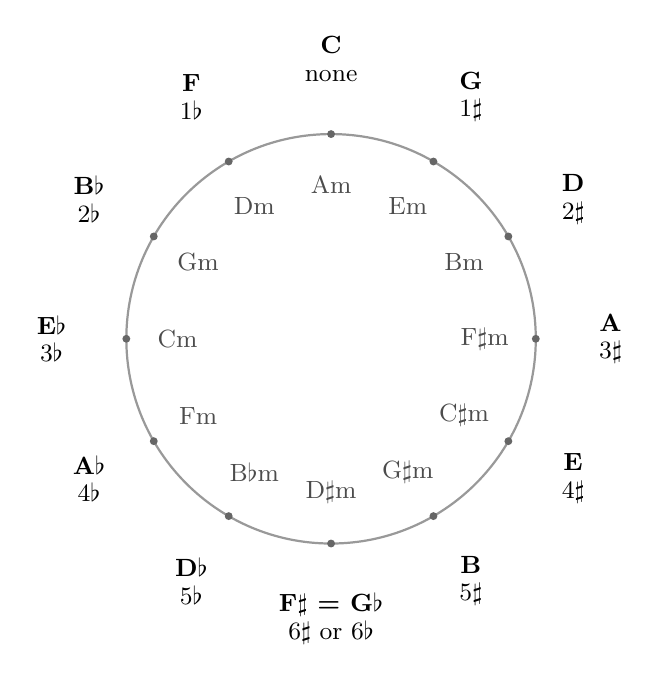
\begin{tikzpicture}
  \draw[black!40, thick] (0,0) circle (2.6);
  \foreach \i/\maj/\acc/\mi in {
    0/C/{none}/Am,
    1/G/{1$\sharp$}/Em,
    2/D/{2$\sharp$}/Bm,
    3/A/{3$\sharp$}/{F$\sharp$m},
    4/E/{4$\sharp$}/{C$\sharp$m},
    5/B/{5$\sharp$}/{G$\sharp$m},
    6/{F$\sharp$ = G$\flat$}/{6$\sharp$ or 6$\flat$}/{D$\sharp$m},
    7/{D$\flat$}/{5$\flat$}/{B$\flat$m},
    8/{A$\flat$}/{4$\flat$}/Fm,
    9/{E$\flat$}/{3$\flat$}/Cm,
    10/{B$\flat$}/{2$\flat$}/Gm,
    11/F/{1$\flat$}/Dm} {
    \pgfmathsetmacro{\a}{90-\i*30}
    \fill[black!60] (\a:2.6) circle (0.05);
    \node[font=\small, align=center] at (\a:3.55) {\textbf{\maj}\\[-1pt]\acc};
    \node[font=\small, text=black!70] at (\a:1.95) {\mi};
  }
\end{tikzpicture}
\caption{The circle of fifths. Going clockwise, each key is a fifth higher and has one more sharp (or one fewer flat). Inside each major key is its relative minor.}
\label{fig:circle-of-fifths}
\end{figure}

Going the other way, counterclockwise, each step moves down a fifth and adds one flat: C, F, B\fl, E\fl, A\fl, D\fl, G\fl. At the bottom of the circle the two directions meet: F\sh{} major and G\fl{} major use exactly the same piano keys, named differently.

\subsection*{A map of neighbors}

Two keys next to each other on the circle share six of their seven notes. That is why music often moves to a neighboring key: so little changes that the move sounds like a short trip.

Keys far apart on the circle, such as C and F\sh, share few notes. Moving between them sounds far more surprising.

The relative minors sit inside the circle, next to their major partners. A minor is inside C, E minor inside G, and so on. A relative minor has the same sharps or flats as its major partner.

\subsection*{Which sharps, which flats}

Sharps always appear in the same order: F\sh, C\sh, G\sh, D\sh, A\sh, E\sh, B\sh. A key with two sharps has the first two, F\sh{} and C\sh. A key with three sharps has F\sh, C\sh{} and G\sh, and so on.

Flats appear in the reverse order: B\fl, E\fl, A\fl, D\fl, G\fl, C\fl, F\fl. A key with three flats has B\fl, E\fl{} and A\fl.

Two facts help you check. In a sharp key, the newest sharp is the seventh note of the scale, a half step below the tonic: in D major, C\sh{} is a half step below D. In a flat key, the newest flat is the fourth note: in F major, B\fl{} is the fourth note.

\begin{curiousbox}
Why does stepping by fifths visit all twelve keys before coming back? Number the keys 0 to 11 around the clock (C = 0, C\sh{} = 1, and so on up to B = 11). A fifth adds 7, and we wrap around after 12, as on a clock.

Starting at 0, the steps give 0, 7, 2, 9, 4, 11, 6, 1, 8, 3, 10, 5, and then 0 again: all twelve numbers. This happens because 7 and 12 have no common factor except 1; in symbols, $\gcd(7, 12) = 1$.

Compare stepping by 3 (a minor third): 0, 3, 6, 9, 0. It returns after only four steps, because 3 divides 12. Stepping by 4 (a major third) visits only three keys. Only steps of 1, 5, 7 and 11 half steps visit every key, and 5 and 7 give the two directions around the circle of fifths.
\end{curiousbox}

\begin{summarybox}
\begin{itemize}
  \item A \emph{scale} is a set of notes in order. Its home note is the \emph{tonic}.
  \item The \emph{major scale} follows the pattern W W H W W W H (W = whole step, H = half step): two matching halves, W W H, joined by a W. The last half step, from the seventh note up to the tonic, is what makes the tonic sound like home.
  \item A major scale uses each letter once. That rule decides whether a black key is called a sharp or a flat.
  \item A piece in a musical \emph{key}, such as the key of G, uses the notes of that major scale and treats its tonic as home.
  \item C major scale fingering, right hand going up: 1--2--3, thumb under, 1--2--3--4--5. G major uses the same fingers.
  \item The \emph{relative minor} starts on the sixth note of a major scale (3 half steps below the tonic) and uses the same notes. Minor sounds darker because its third note is only 3 half steps above the tonic.
  \item The \emph{pentatonic scale} has five notes and no half steps. The black keys form one.
  \item On the \emph{circle of fifths}, each step clockwise adds a sharp and each step counterclockwise adds a flat. Neighbors share six of seven notes.
\end{itemize}
\end{summarybox}

\section*{Exercises}

\begin{exercise}
Build the E major scale with the pattern W W H W W W H. Which notes are black keys?
\end{exercise}

\begin{answerbox}
Start on E. Whole step to F\sh{} (E to F is only a half step, so a whole step skips F), whole step to G\sh, half step to A. Whole step to B. Whole step to C\sh, whole step to D\sh, half step to E. The scale is E, F\sh, G\sh, A, B, C\sh, D\sh, E, with four black keys: F\sh, G\sh, C\sh{} and D\sh{} \listen{E4 F#4 G#4 A4 B4 C#5 D#5 E5:2}.
\end{answerbox}

\begin{exercise}
Build the B\fl{} major scale, using each letter once. How many flats does it have?
\end{exercise}

\begin{answerbox}
Start on B\fl. Whole step to C (skipping B), whole step to D, half step to E\fl. Whole step to F. Whole step to G, whole step to A, half step to B\fl. The scale is B\fl, C, D, E\fl, F, G, A, B\fl{} \listen{Bb3 C4 D4 Eb4 F4 G4 A4 Bb4:2}. It has two flats, B\fl{} and E\fl. We call the fourth note E\fl{} and not D\sh{} because the scale already has a D and needs an E.
\end{answerbox}

\begin{exercise}
Find the relative minor of (a) G major, (b) F major, (c) D major. Write out the notes of (c).
\end{exercise}

\begin{answerbox}
Count down 3 half steps from each tonic, or take the sixth note of the major scale. (a) E minor. (b) D minor. (c) From D, down 3 half steps: C\sh, C, B. So B minor. It uses the notes of D major starting on B: B, C\sh, D, E, F\sh, G, A, B \listen{B3 C#4 D4 E4 F#4 G4 A4 B4:2}.
\end{answerbox}

\begin{exercise}
Use the order of sharps and flats. (a) A major has three sharps; which ones? (b) E\fl{} major has three flats; which ones?
\end{exercise}

\begin{answerbox}
(a) The first three sharps: F\sh, C\sh{} and G\sh. Check: G\sh{} is a half step below A, the tonic. (b) The first three flats: B\fl, E\fl{} and A\fl. Check: A\fl{} is the fourth note of E\fl{} major (E\fl, F, G, A\fl).
\end{answerbox}

\begin{exercise}
Which single note is different between (a) C major and G major, (b) C major and F major? Where are these keys on the circle?
\end{exercise}

\begin{answerbox}
(a) F in C major becomes F\sh{} in G major. (b) B in C major becomes B\fl{} in F major. G and F are the two neighbors of C on the circle, one on each side, which is why each differs from C by one note.
\end{answerbox}
